\documentclass[a4paper, twocolumn, 11pt, twoside]{article}

% update your language here.
\usepackage[portuges]{babel}
\usepackage{linguamatica}

% added packages
\usepackage{comment}
\usepackage{makecell} % for formating column heads
\renewcommand\theadfont{\bfseries}
\usepackage{subfig}
\usepackage{graphicx} % http://ctan.org/pkg/graphicx
\usepackage{listings} % see below
\renewcommand{\lstlistingname}{Algorithm}% rename caption: Listing -> Algorithm
\usepackage{color}
\usepackage{multirow}
%\usepackage{coffee}

%% Please use UTF8 in your document

%% Set the bibliography style.
%% Styles provided for Spanish (Castilian), Catalan and Portuguese.
%% Other languages will be created on a required basis.

\bibliographystyle{sp_por}   % This for Portuguese
% \bibliographystyle{sp_esp} % This for Castilian
% \bibliographystyle{sp_cat} % This for Catalan


%% You can leave this unchanged. It will be updated by the editors when your paper gets published.
\submitted{15 de \OCT{} 2017}
\accepted{3 de \DEC{} 2017}


%% Add your title in the main language used in the article
\title{Explorando Relações de Apoio e Oposição \\em Títulos de Notícias de Política}

%% Currenty the title in English is also mandatory
\titleEN{Exploring Support and Opposition Relationships in Portuguese Political News Headlines}


%% Add authors here. Three lines for each author.
%% First line with author name, second with the affiliation and third with e-mail
%% In cases where a second line is needed for the affiliation, use the command \nl to separate them. 
\author{
  David S. Batista \\
  %\instituto{Comtravo GmbH}
  \email{dsbatista@gmail.com} 
}


\begin{document}
\maketitle

%% Add the abstract in the main language for the article. If possible, doesn't add any citations here.
\begin{resumo}
Os títulos de notícias de política relatam com frequência interacções envolvendo personalidades políticas, sendo que  muitas dessas interacções correspondem a uma uma relação de apoio ou de oposição de uma personalidade para uma outra personalidade.

{\bf TODO: desenvolver}

Neste trabalho, analisámos centenas de milhares de títulos de notícias de artigos arquivados, identificando aqueles que expressam uma relação de apoio ou oposição entre duas personalidade políticas. Além de detectar a relação também associamos os nomes das personalidades políticas com a sua entrada na Wikidata. Este processo resulta num grafo de relações de apoio e oposição entre personalidades políticas, cobrindo um período de cerca de 24 anos, permitindo fazer diferentes tipos de interrogações ao grafo envolvendo as personalidades políticas e a sua informação da Wikidata, e.g.: \textit{Que personalidades do BE se opuseram a Jerónimo de Sousa?}, \textit{Que acusações fez Passos Coelho a José Sócrates?}, \textit{Quem de dentro do PS se opôs/apoiou a José Sócrates?}, \textit{Que personalidades afiliadas ao BE se opuseram a personalidades do PCP?}, \textit{Que personalidades do PS apoiaram personalidades do PSD?}, \textit{Que políticos do BE estiveram envolvidos em conflitos internos ao próprio partido?}.

Neste artigo descrevemos em detalhe processo de extracção de relações dos títulos de notícias, tornamos disponível publicamente o grafo que resultou do processo de extracção, bem como a colecção de dados anotada manualmente, que permitiu treinar um classificador de aprendizagem estatística para identificar as relações. Também descrevemos um \textit{website} onde é possível explorar o grafo de forma interactiva bem como fazer interrogações envolvendo personalidades políticas e partidos.

\end{resumo}

%% Add keywords in the article main language, in lowercase
\palavraschave{web semântica, RDF, PLN, relações semânticas, ciência política, dados anotados}



\newpage



%% Add the abstract in English
\begin{abstract}
Politics news headlines often report information involving political personalities. In this paper, we analysed hundreds of thousands of archived article news titles, identifying those that express a relationship of support or opposition between two political personalities. Besides detecting the relationship we also associate the names of the political personalities with their Wikidata entry. This process results in a graph of support and opposition relations between political personalities, covering a period of about 24 years, allowing to make different types of interrogations to the graph involving the political personalities and their Wikidata information, e.g.: \textit{Which BE personalities opposed Jerónimo de Sousa? }, \textit{Which accusations did Passos Coelho make to José Sócrates?}, \textit{Who from within the PS opposed/supported José Sócrates?}, \textit{Which personalities affiliated to BE opposed personalities from the PCP?}, \textit{Which personalities from the PS supported personalities from the PSD?}, \textit{Which BE politicians were involved in internal conflicts within the party itself?}.

In this paper we describe in detail process of extracting relations from news headlines, we make publicly available the graph that resulted from the extraction process, as well as the manually annotated data collection that allowed training a statistical learning classifier to identify relations. We also describe a \textit{website} where one can interactively explore the graph as well as make interrogations involving political personalities and parties.
\end{abstract}

%% add the keywords in English
\keywords{semantic web, RDF, NLP, semantic relationships, political science, annotated dataset}



\newpage


\section{Introdução}
\label{sec:intro}

Os títulos de notícias relacionados com política ou políticos relatam com frequência interacções envolvendo duas ou mais personalidades políticas. Muitas dessas interacções correspondem a uma relação de apoio ou oposição de uma personalidade para uma outra personalidade. Por exemplo:

\begin{itemize}
\item{\textit{"Sócrates acusa Cavaco de mentir"}}
\item{\textit{"Marques Mendes critica estratégia de Rui Rio"}}
\item{\textit{"Défice. Cristas responsabiliza Costa por possíveis sanções"}}
\end{itemize}

A análise de um grande número deste tipo de relações ao longo do tempo permite vários estudos, por exemplo: encontrar quais as grandes comunidades de apoio ou oposição em função dos governos no poder ou encontrar as grandes alianças e oposições e as suas dinâmicas. Pode-se também explorar individualmente uma personalidade ao longo do tempo, por exemplo, comparando as relações de apoio ou oposição antes de tomar posse num determinado cargo público com as relações depois de ter assumido o cargo, ou ver que relações de apoio subitamente emergiram. Também pode ser usado para rapidamente reunir uma colecção de notícias contendo interacções de apoio ou oposição envolvendo personalidades e partidos políticos específicos, por exemplo, para auxiliar numa tarefa de jornalismo de investigação. Tendo um método automático para extrair estas relações e podendo aplicá-lo a uma colecção de dados abrangendo longos períodos temporais permitiria concretizar os exemplos descritos acima.

Neste trabalho apresentamos um método para extrair relações de apoio ou oposição entre personalidades políticas e descrevemos os resultados da aplicação do mesmo a uma colecção de notícias abrangendo um período de cerca de 25 anos. Durante o processo de extracção das relações ligamos as personalidades políticas envolvidas ao seu identificador na Wikidata~\citep{MKGGB2018}, enriquecendo assim a relação com informação associada à personalidade (e.g.: afiliação política, cargos públicos exercidos, legislaturas, relações familiares, etc.). 

Todas as relações extraídas são representadas sob a forma de triplos semânticos seguindo a norma Resource Description Framework (RDF)~\citep{schreiber2014primer}. As personalidades políticas envolvidas, representadas pelo seu identificador na Wikidata, são ligadas através de uma relação de oposição ou apoio representada pela notícia que dá suporte à relação, dando assim origem a um gráfico semântico. Desta forma é então possível formular interrogações SPARQL~\citep{2013sparql} envolvendo a informação da Wikidata associada a cada personalidade e as relações extraídas dos títulos de notícias, por exemplo:

\begin{itemize}
\item{Listar todas as notícias onde a personalidade X se opõe à personalidade Y}
\item{Listar os membros de um determinado partido que apoiaram alguma personalidade específica}
\item{Lista de membros de um determinado partido apoiados/opostos membros de outro partido}
\item{Lista de membros de um determinado partido apoiados/opostos membros do mesmo partido}
\item{Lista de personalidades que estão ligadas através de uma relação familiar e de uma relação de oposição/apoio}
\item{Lista de personalidades que fazem parte do mesmo Governo e que estão envolvidas numa relação de oposição/apoio}
\end{itemize}

As principais contribuições deste trabalho são: 

\begin{itemize}
\item{um gráfico semântico RDF ligando personalidades políticas representadas na Wikidata através de uma relação de oposição ou apoio suportada por uma notícia}
\item{um conjunto de dados anotados utilizado para treinar os classificadores de extração das relações de títulos de notícias, e ligar as personalidades mencionadas à Wikidata}
\item{um interface web que permite explorar o gráfico semântico, permitindo filtrar o tipo de relações, o período de tempo das notícias, e o peso de uma relação, ou seja, o número de noticias que suportam uma relação entre duas personalidades.}
\end{itemize}

Este artigo está organizado da seguinte forma: na Secção~\ref{sec_related_work} referimos trabalho relacionado, na Secção~\ref{sec_kb} descrevemos a Base de Conhecimento usado no suporte de ligação das personalidades políticas à Wikidata. A Secção~\ref{sec:data_sources} refere e descreve as fontes de notícias utilizadas. Na Secção~\ref{sec:rel_data_annot} detalhamos o conjunto de dados anotados e na Secção~\ref{sec:classifiers} os classificadores de aprendizagem supervisionada desenvolvidos. Na Secção~\ref{sec:pipeline} descrevemos o processo extracção de triplos e a construção do gráfico semântico. Finalmente, na Secção~\ref{sec:future_work} apresentamos ideias futuras para melhorar e continuar este trabalho.


\section{Trabalho Relacionado}
\label{sec_related_work}

A análise de sentimento no contexto de processamento de linguagem natural (PLN) tem sido maioritariamente alvo de estudo em conteúdo gerado em redes redes sociais~\citep{10.1145/3185045} ou na avaliação de produtos ou serviços~\citep{pontiki-etal-2016-semeval}. Nestes domínios o autor do texto e o alvo da opinião são explícitos. No entanto este tipo de abordagem não se aplica no contexto de análise de notícias de política, onde existe com frequência um sentimento expresso entre actores políticos sob a forma de relações de apoio ou oposição~\citep{balahur2009opinion, balahur-etal-2010-sentiment}.

% Who Blames or Endorses Whom? Entity-to-Entity Directed Sentiment Extraction in News Text
% https://aclanthology.org/2021.findings-acl.358/
Alguns trabalhos exploram relações com sentimento positivo ou negativo entre entidades mencionadas em notícias. \cite{park-etal-2021-blames} define a tarefa de extracção de sentimento direccionada como: dada uma frase $s$ referindo duas entidades $p$ e $q$, detectar qual a relação de sentimentos entre $p$ e $q$ de entre cinco possíveis: neutra, $p$ tem uma opinião positiva ou negativa em relação a $q$, ou $q$ tem uma opinião positiva ou negativa em relação a $p$.

% Os autores propõem resolver propõem uma abordagem simples mas eficaz de abordar o problema da extracção de sentimentos dirigida, a que chamamos DSE2QA; transformamos a tarefa tarefa extracção de sentimento direccionado em sub-tarefas que visam responder a perguntas de sim/não sobre se um sentimento alvo está incorporado no texto. A ideia básica é perguntar a uma máquina inteligente que possa responder sim/não a perguntas sobre se existe um sentimento alvo e depois combinar as respostas correspondentes a cada classe de sentimento para fazer um palpite final. 

\cite{liang2019blames} define a tarefa de extração de relações de culpabilidade: dado um artigo $d$ e um conjunto de entidades $e$, detectar se existe uma relação de culpabilidade $(s,t)$, onde $s \in e$ e $t \in e$, quando $s$ culpa $t$ com base no artigo $d$, sendo que há $|e| \cdot (|e| - 1)$ possíveis relações de culpabilidade, .

% https://aclanthology.org/P13-1108/
% https://aclanthology.org/N19-1167/

Outros autores exploram estas relações num contexto de política internacional entre nações. \cite{oconnor-etal-2013-learning} propõem um modelo não supervisionado baseado em \textit{topic models}~\cite{} extraindo eventos ocorridos num determinado período de tempo envolvendo duas nações, e não um conjunto fechado de relações. \cite{han-etal-2019-permanent} geram de forma não supervisionada descritores de relações para pares de nações mencionadas em notícias recorrendo a \textit{embeddings} usados para ordenar o text que descreve a relação.

% take a set of documents and nation entity pairs as inputs and generate relationship descriptors for the entity pairs in an unsupervised setting. They are both trained in an encoder-decoder style training process in an unsupervised manner. Given new text with an entity pair, they generate d descriptor embeddings that are used to rank candidate descriptors.

No contexto de análise de notícias de política em Português, e tanto quanto é do meu conhecimento, julgo este ser um dos primeiros trabalhos a propor um método para extrair de forma automática relações de apoio e oposição entre personalidades políticas de forma a poder construir um grafo semântico.

% 2006
% \citep{thomas-etal-2006-get} investigate whether one can determine from the transcripts of U.S. Congressional floor debates whether the speeches represent support of or opposition to proposed legislation. 
%  determine from the transcripts of U.S. Congressional floor debates whether each “speech” (continuous single-speaker segment of text) represents support for or opposition to a proposed piece of legislation.
% https://aclanthology.org/W06-1639.pdf


% https://aclanthology.org/W15-5614/ - An Annotated Corpus for Sentiment Analysis in Political News
% https://www.sciencedirect.com/science/article/pii/S1877050921018755


% 2017
% We propose a deep learning architecture to capture argumentative relations of attack and support from one piece of text to another, of the kind that naturally occur in a debate.
% Proceedings of the 2017 Conference on Empirical Methods in Natural Language Processing, pages 1374–1379Copenhagen, Denmark, September 7–11, 2017. c©2017 Association for Computational LinguisticsIdentifying attack and support argumentative relations using deep learning
% https://aclanthology.org/D17-1144.pdf


\begin{table*}[!h]
  \centering
  \begin{tabular}{lc}
      {\bf Título} & {\bf Relação} \\
      \hline
	  \textbf{Sá Fernandes} acusa \textbf{António} Costa de defender interesses corporativos &	Ent\textsubscript{1}-opõe-se-Ent\textsubscript{2} \\
	  \textbf{Passos Coelho} é acusado de imaturidade política por \textbf{Santos Silva} &	Ent\textsubscript{2}-opõe-se-Ent\textsubscript{1}	\\
	  \textbf{Manuel Alegre} apoia candidatura de \textbf{Maria de Belém} &	Ent\textsubscript{1}-apoia-Ent\textsubscript{2}	\\
	  \textbf{Manuel Alegre} recebe apoio de \textbf{Jorge Sampaio} & Ent\textsubscript{2}-apoia-Ent\textsubscript{1}	\\
	  \textbf{Rui Tavares} e \textbf{Ana Drago} eleitos nas primárias do LIVRE & outra	\\
	  \textbf{Teresa Zambujo} reconhece vitória de \textbf{Isaltino Morais} & outra	\\
	  CDS acusa \textbf{Marcelo Rebelo de Sousa} de pôr em causa relação com \textbf{Cavaco} & outra \\
	  \hline
  \end{tabular}
  \caption{Exemplos de títulos e das relações manualmente anotadas correspondentes.}
  \label{tab:samples}
\end{table*}


\section{Base de Conhecimento}
\label{sec_kb}
Dado que as personalidades envolvidas nas relações a extrair são personalidades políticas relevantes, começámos por construir uma Base de Conhecimento usando a Wikidata~\citep{MKGGB2018}. Fazendo interrogações SPARQL~\cite{2013sparql} ao seu \textit{endpoint} público~\footnote{\url{https://query.wikidata.org/sparql}} recolhemos o identificador de todas as:

\begin{itemize}  
\item pessoas que são ou foram afiliadas a algum partido político português
\item pessoas portuguesas nascidas depois de 1935 cuja profissão seja: \textit{juiz, economista, advogado, funcionário público, político, empresário ou banqueiro}
\item pessoas que têm ou tiveram pelo menos um cargo de uma lista de cargos públicos portugueses previamente seleccionados (e.g.: \textit{ministro, líder do partido, embaixador}, etc.)
\end{itemize}  

Para além dos resultados destas interrogações, seleccionámos manualmente alguns identificadores de personalidades não abrangidos pelas interrogações SPARQL definidas acima. Acrescentamos também todos os identificadores de partidos políticos a que as personalidades possam estar afiliadas. Este processo resultou num total de {\bf XXX} personalidades e de {\bf XXX} partidos políticos. Descarregamos depois a página na Wikidata para cada um dos identificadores recolhidos, utilizando um outro \textit{endpoint}\footnote{\url{https://www.wikidata.org/wiki/Special:EntityData?}} público.

Para cada personalidade política, seleccionámos o seu identificador na Wikidata, o seu nome mais comum e os nomes alternativos, por exemplo combinações de nomes próprios e apelidos. Com base nestes três campos, criámos um índice no ElasticSearch~\citep{10.5555/2904394} usando a sua configuração de omissão, não fazendo uso de qualquer funcionalidade extra tais como analisadores de $n$-gramas.


\section{Fontes de dados}
\label{sec:data_sources}

A principal fonte de notícias foi o arquivo da web portuguesa~\citep{SearchPastPWA2013}. Usando a \textit{API} pública de pesquisa recolhemos páginas arquivadas restringindo os resultados a ocorrências de nomes reunidos na Secção~\ref{sec_kb} e a 45 domínios \texttt{.pt} associados a diversas fontes de informação: jornais \textit{on-line}, \textit{websites} de estações de televisão e rádio, e portais agregadores de conteúdos. 

Uma segunda fonte de notícias foi a colecção CHAVE\footnote{\url{https://www.linguateca.pt/CHAVE/}}~\citep{DBLP:conf/clef/SantosR04, santos-rocha-2001-evaluating}, contendo os artigos do jornal PÚBLICO publicados entre 1994 e 1995. Finalmente, também acrescentámos alguns artigos não arquivados pelo arquivo.pt, retirados directamente das secções {\it Mundo}, {\it Política} e {\it Sociedade} do site publico.pt. 

Deste processo resultou uma colecção de cerca de \textbf{XXXX} milhões de artigos publicados entre 1994 e \textbf{XXXX}. De seguida foi aplicado um pré-processamento de modo a remover notícias com: títulos duplicados, títulos com menos de 4 palavras, e títulos ou URL contendo palavras de uma lista pré-definida (e.g.: desporto, celebridades, artes, cinema) que sugerem um o outro contexto que não política. Este pré-processamento resultou em \textbf{XXXX} milhões de títulos, cerca de \textbf{XXXX}\% dos dados inicialmente recolhidos.

% A grande maioria das notícias tem como origem o arquivo da web portuguesa, através da sua \textit{API} que retorna o título e o HTML original da página. Limpar os dados, de forma a descartar todo o HTML e ter o corpo da notícia não é uma tarefa simples, especialmente considerando o variedade de domínios e o período temporal. Por esta razão optamos por focar a extracção de relações no título das notícias.


\section{Colecção de Relações Anotadas}
\label{sec:rel_data_annot}

De forma a poder treinar classificadores de aprendizagem supervisionada para identificar automáticamente as relações presentes nos títulos das notícias, e fazer a ligação das personalidades com a Wikidata, anotámos manualmente um conjunto de títulos com: as personalidades, os identificadores na Wikidata e a relação entre as personalidades.

Começamos por pré-processar todos os títulos automáticamente. Usando o pacote de software spaCy 3.0~\citep{spacy} e com o modelo~\texttt{pt\_core\_news\_lg-3.0.0} fizemos o reconhecimento de entidades mencionadas do tipo \texttt{PESSOA}, para cada entidade reconhecida tentamos encontrar o seu identificador correspondente na Wikidata fazendo uma interrogação ao índice descrito na Secção~\ref{sec_kb} e assumindo que na lista de resultados o primeiro é o identificador correcto associado à entidade. Seleccionámos depois apenas títulos referindo duas pessoas e ambas com um identificador Wikidata associado.

Fomos depois seleccionando títulos para anotação. Sempre que necessário corrigimos as entidades reconhecidos e o identificador na Wikidata, e anotamos a relação existente: \textbf{oposição} ou \textbf{apoio}, e a direcção da mesma. Quando nenhuma das duas se verifica a relação é anotada como \textbf{outra}. A Tabela~\ref{tab:samples} demonstra alguns exemplos das relações anotadas.

Este processo resultou num conjunto de dados contendo 3.324 títulos anotados e {\bf XXXX} personalidades políticas. A Tabela~\ref{tab:rel_dataset} caracteriza os dados em termos de número de relações e direcção. É de notar que a maioria dos títulos contém uma relação de \textbf{oposição} ou \textbf{outra}, e a grande maioria as relações têm uma direcção da primeira para a segunda entidade, Ent\textsubscript{1}$\rightarrow$Ent\textsubscript{2}.

% jq -r '"\(.label)"' < politiquices_data_v3.0.jsonl | sort | uniq -c

\begin{table}[!h]
    \begin{center}
    \begin{tabular}{l ccr}
        {\bf Relação} & {\bf \footnotesize{Ent\textsubscript{1}$\rightarrow$Ent\textsubscript{2}}} & {\bf \footnotesize{Ent\textsubscript{2}$\rightarrow$Ent\textsubscript{1}}} & {\bf Total} \\
        \hline
        opõe-se          &  1 155  &  102  &  1 257  \\
        apoia            &    717  &   44  &    761  \\
        outra            &    -    &   -   &  1 306  \\
		\hline
		Total			 &  1 872  &  146  &  3 324  \\
    \end{tabular}
	\caption{Relações por classe e direcção.}
	\label{tab:rel_dataset}
	\end{center}
\end{table}

{\bf TODO: tabela aqui e referir as entidades ligadas à Wikidata}


\begin{comment}
\begin{table}
    \begin{center}
    \begin{tabular}{l r}
	\multicolumn{2}{c}{\bfseries Named-Entities (surface strings)} \\
	\hline
    Nr. Named-Entities                 &  5 348  \\
    Nr. Unique Named-Entities          &    754  \\
    \ \ - with a Wikidata entry		   &    631  \\
    \ \ - without a Wikidata entry     &    129  \\
                                       &         \\
	\multicolumn{2}{c}{\bfseries Named-Entities per Wikidata entry} \\
	\hline
	Mean      						   &  1.387 \\
	Std. Dev. 						   &  0.614 \\
	Mode      						   &  1 \\
	Median   						   &  1 \\   
    \hline
    \end{tabular}
	\caption{Named-Entities and Wikidata entries.}
	\label{tab:named_entities_linked}
	\end{center}
\end{table}
\end{comment}


\section{Processo de Extracção de Relações}
\label{sec:classifiers}

O processo de extração de triplos em formato Resource Description Framework (RDF)~\citep{schreiber2014primer} a partir dos títulos das notícias envolve 4 componentes, nomeadamente: reconhecimento de entidades-mencionadas, ligação das entidades com um identificador da Wikidata presente na Base de Conhecimento (BC), classificação do tipo de relação e da sua direcção. Nesta secção descrevemos em detalhe cada um destes componentes.


\subsection{Reconhecimento de Entidades}
\label{subsec:ner}

O reconhecimento de entidades mencionadas é baseado num método híbrido combinando regras com um modelo supervisionado. 

Usando a componente \texttt{EntityRuler}\footnote{\url{https://spacy.io/usage/rule-based-matching}} do spaCy 3.0, definimos uma série de regras combinando padrões baseados nos nomes de todas as personalidades da BC. Para detectar as entidades do tipo pessoa este classificador aplica primeiro as regras e de seguida o modelo supervisionado para Português do spaCy.

\textbf{TODO: quem decide o que é final? as regras ou o modelo?}

A Tabela~\ref{tab:results_ner} mostra a performance para as 3 abordagens sob o conjunto de dados anotado, contendo {\bf XXXX} personalidades políticas.

\begin{table}[!h]
    \begin{center}
    \begin{tabular}{l ccc}
		{\bf Abordagem}  & {\bf P} & {\bf A} & {\bf F\textsubscript{1}} \\
        \hline
        Regras           &  0.99     &  0.42     & 		0.59		\\
        Modelo           &  0.97     &  0.91     & 		0.94		\\
		Regras+Modelo    &  0.97     &  0.92     & 		0.94		\\
    \end{tabular}
	\caption{ (P)recisão, A(brangência) e F\textsubscript{1} para a componente de REM combinando regras e o modelos supervisionado.}	
	\label{tab:results_ner}
	\end{center}
\end{table}


\subsection{Ligação com a Wikidata}
\label{subsec:ent_linking}

O procedimento para ligar as personalidades com a Wikidata tenta primeiro encontrar o identificador da Wikidata correcto na BC analisando apenas o título da notícia, se este processo falhar, tenta usar possíveis referências à mesma personalidade no texto da notícia.

Numa primeira fase o algoritmo começa por gerar uma lista de candidatos, para uma determinada personalidade usando a BC. Se a lista contem apenas um candidato e a similaridade Jaro~\citep{jaro1989} entre a personalidade e o candidato é de pelo menos 0,8 esse candidato é seleccionado. Se houver mais do que um candidato o algoritmo filtra apenas aqueles com uma similaridade de 1,0 e se houver apenas um esse é o candidato seleccionado. 

Se nenhum candidato for gerado na primeira fase, o algoritmo tenta expandir as entidades mencionadas no título com base no texto da notícia, explorando o padrão em que uma personalidade mencionada no título por um versão curta do seu nome é também referida no texto da notícia por um nome mais completo. \textbf{TODO: adicionar um exemplo}

O algoritmo começa por identificar todas as pessoas mencionadas no texto da notícia, usando a componente descrita na secção~\ref{subsec:ner} descartando todas que não têm pelo menos um nome em comum com a personalidade a ser desambiguada.  Se do processo de expansão resulta mais do que uma entidade expandida, escolhemos o candidato da BC  com uma similaridade 1.0 para com a entidade expandida, se existir. 

Se do processo resulta apenas uma entidade expandida e se há uma similaridade de 1.0 com apenas um dos candidatos anteriormente seleccionados da BC, esse candidato é escolhido. 

Caso contrário a entidade expandida é usada para recolher uma nova lista de candidatos da BC, se nessa lista apenas há um candidato e a sua similaridade Jaro é de pelo menos 0.8 com a entidade expandida, esse candidato é escolhido. Se há mais do que um candidatos e apenas um tem uma similaridade 1.0 com a entidade expandida esse é escolhido. Em qualquer outro caso nenhum candidato é retornado.

% A figura~\ref{fig:entity_linking} mostra um exemplo.

% Algoritmo~\ref{lst:alg3} descreve esta segunda abordagem em pseudo-código python.{lst:alg3}


% TODO: algoritmo
\begin{comment}
\begin{lstlisting}[language=python,columns=fullflexible,label={lst:alg1},caption=Entity-Linking approach.]]
def entity_linking(person, url):
    candidates = get_candidates(person)
    wiki_id = title_only(person, candidates)
    if not wiki_id:
        news_text = get_text(text)
        expanded = expand_entity(person, news_text)
        wiki_id = article_text(person, candidates, expanded)
    return wiki_id
\end{lstlisting}
\end{comment}

\begin{comment}
\begin{lstlisting}[language=python,columns=fullflexible,label={lst:alg2},caption=Headline approach.]]
def title_only(person, candidates):
    wiki_id = None
    if len(candidates) == 1:
        if fuzzy(person,candidades[0]):
            wiki_id = candidates[0]
    else:
        if len(matches := exact(person, candidates)) == 1:
            wiki_id = candidates[0]
    return wiki_id
\end{lstlisting}
\end{comment}

\begin{comment}
\begin{lstlisting}[language=python,columns=fullflexible,label={lst:alg3},caption=News text approach.]]
def article_text(expanded, candidates):
    if len(expanded) == 1:
        per_expanded = expanded[0]
        matches = exact(per_expanded, candidates)
        if len(matches) == 1:
            return matches[0]

        new_candidates = get_candidates(expanded)
        if len(new_candidates) == 1:
            if fuzzy(per_expanded, new_candidates[0]):
                return candidates[0]
 
        matches = exact(per_expanded, new_candidates)
    	if len(matches) == 1:
            return matches[0]

    if len(expanded) > 1:
        exact_matches = []
        for e in expanded:
            exact_matches.extend(exact(e, candidates))
    	if len(matches) == 1:
            return matches[0]

    return None
\end{lstlisting}
\end{comment}

% TODO: figuras
\begin{comment}
\begin{figure}
\centering

\subfloat{
	\label{subfig:correct}
	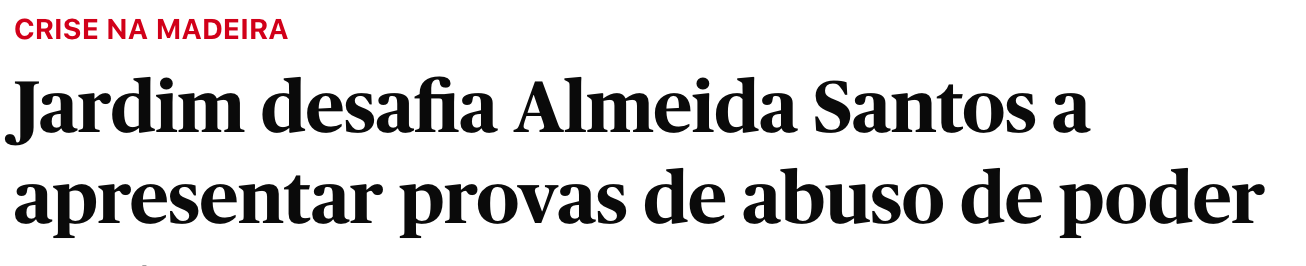
\includegraphics[width=0.45\textwidth]{entity_linking_title.png} } 

\subfloat{
	\label{subfig:notwhitelight}
	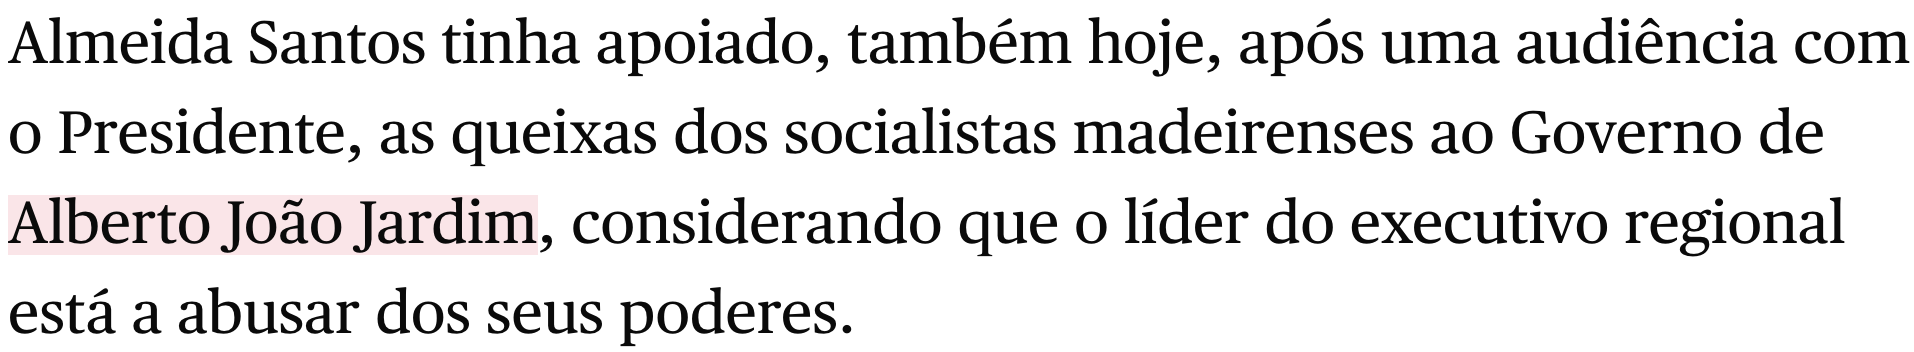
\includegraphics[width=0.45\textwidth]{entity_linking_body} } 
	
\caption{The same person \textit{Jardim}, mentioned in the headline and body, with different surface strings.}
\label{fig:entity_linking}

\end{figure}
\end{comment}

Os resultados desta abordagem sobre o conjunto de dados anotados e descritos na Secção~\ref{sec:rel_data_annot} são descritos na Tabela~\ref{tab:ent_linking_results}. A classificação \textit{incorrecta} corresponde a personalidades que não foram associadas ao identificador correcto na Wikidata, \textit{não desambiguada} para as que o algoritmo não conseguiu chegar a um identificador único ou não encontrou nenhum identificador na BC.

São relatadas duas avaliações diferentes, Eval. 1 são os resultados para o algoritmo, tal como descrito acima. Eval. 2 é o mesmo algoritmo mas com dois mapeamentos baseados em contagens à priori sobre todas as notícias recolhidas, concretamente: \textit{Cavaco} para \textit{Cavaco Silva} e \textit{Marques Mendes} para \textit{Luís Marques Mendes}.

\textbf{TODO: explicar como foram feitas as contagens à priori}


\begin{table}
    \begin{center}
    \begin{tabular}{l rr}
        {\bf Classificação} & {\bf Eval. 1} & {\bf Eval. 2} \\
        \hline
        correcta            &   5059        &  5136    \\
        incorrecta          &     43        &    43    \\
		não desambiguada    &    246        &   169    \\    
        \hline
		{\bf Exactidão }    &  0.934	    &  0.958   \\
    \end{tabular}
	\caption{Resultados da avaliação do algoritmo de ligação com a Base de Conhecimento.}
	\label{tab:ent_linking_results}
	\end{center}
\end{table}


\subsection{Classificador de Tipo de Relação}
\label{subsec:rel_classifier}

Decidimos decompor a tarefa de classificação do tipo de relação, descritas na Tabela~\ref{tab:rel_dataset}, em dois classificadores diferentes: um classificador para o tipo de relação e outro para a direcção da relação, por oposição a treinar um único classificador que teria que distinguir de entre 5 classes. Esta secção descreve o classificador do tipo de relação presente num título, tendo 3 classes possíveis: \textbf{opõe-se}, \textbf{apoia} e \textbf{outra}.

Os dados foram divididos em 4 partições, de forma a podermos fazer uma avaliação cruzada. 

\begin{table}[!h]
    \begin{center}
    \begin{tabular}{l cccr}
        {\bf Relação} & {\bf P\textsubscript{1}}&  {\bf P\textsubscript{2}}  & {\bf P\textsubscript{3}} & {\bf P\textsubscript{4}} \\
        \hline
        opõe-se          &  xxx  &  xxx  &  xxx  & xxx \\
        outra            &  xxx  &  xxx  &  xxx  & xxx \\
        apoia            &  xxx  &  xxx  &  xxx  & xxx \\
		\hline
    \end{tabular}
	\caption{Número de relações por partição}
	\end{center}
\end{table}


Experimentamos e avaliámos diferentes abordagens para classificação supervisionada das relações presentes nos títulos, nomeadamente: um classificador SVM~\citep{cortes1995support} com um kernel linear, uma rede neuronal recorrente do tipo LSTM~\citep{10.1162/neco.1997.9.8.1735}, e uma rede neural do tipo \textit{transformer}, o DistilBERT~\citep{9463516}.


Para o SVM utilizámos como \textit{features} uma abordagem baseada em vectores TF-IDF~\citep{DBLP:journals/ipm/SaltonB88}.


\begin{table}[!h]
    \begin{center}
    \begin{tabular}{l ccc}
		\multicolumn{4}{c}{SVM}\\
		\hline
        {\bf Relação} & {\bf P} & {\bf A} & {\bf F\textsubscript{1}} \\
		\hline
        opõe-se          &  0.71  &  0.69  &  0.70   \\
        outra            &  0.69  &  0.69  &  0.69   \\
        apoia            &  0.65  &  0.69  &  0.67   \\
		\hline
		Macro-Média      &	0.69  &  0.69  &  0.69   \\
    \end{tabular}
	%\caption{(P)recisão, A(brangência) e F\textsubscript{1} para uma avaliação com 4-partições e validação cruzada.}
	\end{center}
\end{table}


\begin{table}[!h]
    \begin{center}
    \begin{tabular}{l ccc}
		\multicolumn{4}{c}{bi-LSTM}\\
		\hline
        {\bf Relação} & {\bf P} & {\bf A} & {\bf F\textsubscript{1}} \\
		\hline
        opõe-se          &  0.75  &  0.64  &  0.69   \\
        outra            &  0.65  &  0.75  &  0.70   \\
        apoia            &  0.65  &  0.62  &  0.63   \\
		\hline
		Macro-Média      &  0.69  &  0.68  &  0.68   \\
    \end{tabular}
	\end{center}
\end{table}


\begin{table}[!h]
    \begin{center}
    \begin{tabular}{l ccc}
		\multicolumn{4}{c}{DistilBERT}\\
		\hline
        {\bf Relação} & {\bf P} & {\bf A} & {\bf F\textsubscript{1}} \\
		\hline
        opõe-se          &  0.74  &  0.76  &  0.75   \\
        outra            &  0.72  &  0.71  &  0.72   \\
        apoia            &  0.72  &  0.71  &  0.71   \\
		\hline
		Macro-Média      &  0.73  &  0.72  &  0.72   \\
    \end{tabular}
	\end{center}
\end{table}





% difficulty, challenge due to

% idiomatic expressions
%
% José Lello diz que Nogueira Leite quer "abifar uns tachos"	ent1_opposes_ent2
% Jerónimo de Sousa: Passos Coelho "não dá a cara com a careta"
% Louçã diz que “António Borges é o grilo falante” de Passo Coelho	ent1_opposes_ent2
% Louçã acusa Passos de ser o “cangalheiro da melhor maternidade” do país	ent1_opposes_ent2

% difficult to extract the exact context, syntactic parsing
%
% Socialistas aprovam voto de protesto contra elogios de Jaime Gama a Alberto João Jardim
% Nobre Guedes apela a levantamento popular para impedir entrada de Sócrates em Coimbra

% Francisco Lopes aponta convergência entre Cavaco e Alegre no rumo que levou ao 'afundamento' do país
% oposses both persons

% não anotei felicita qnd ganha eleicoes, nem 


\subsection{Classificador de Direção da Relação}
\label{subsec:rel_direction}

Este classificador tem 2 classes possíveis. O conjunto de dados tem um viés para com a classe Ent\textsubscript{1} $\rightarrow$ Ent\textsubscript{2}, como mostra a Tabela~\ref{tab:rel_dataset} representando 91,5\% dos dados. Assim, optamos por desenvolver uma abordagem baseada em regras para detectar apenas a classe Ent\textsubscript{2}$\leftarrow$Ent\textsubscript{1}, e sempre que nenhuma das regras se verifica o classificador atribui a classe Ent\textsubscript{1} $\rightarrow$ Ent\textsubscript{2} por omissão.

As regras são baseado em padrões construídos com informação morfológica e sintáctica~\citep{nivre-etal-2020-universal} extraída do título com o spaCy e usando o mesmo modelo usado para reconhecimento de nomes de personalidades. Extraímos a informação morfo-sintáctica de todas as palavras, incluindo para os verbos informação sobre a conjugação: a pessoa e o número.

\begin{itemize}

\item \textbf{VOZ\_PASSIVA}: identificamos a presença da voz passiva usando duas regras: verificando se a informação morfológica associado ao verbo principal do título indica a presença da voz passiva, e se for o caso verificamos se a entidade Ent\textsubscript{1} é a cabeça do verbo ligada por uma dependência do tipo \textbf{acl}. A segunda regra verifica se a cabeça da entidade Ent\textsubscript{1} é um verbo ligado por uma dependência do tipo \textbf{nsubj:pass} e se o mesmo verbo é também a cabeça da entidade Ent\textsubscript{2} ligado por uma dependência do tipo \textbf{obl:agent}.

\textbf{TODO: exemplo}

% COMMENT: The head of the acl relation is the noun that is modified, and the dependent is the head of the clause that modifies the noun.%

\item \textbf{VERBO\_ENT2}: é baseada num padrão morfológico, \texttt{<PUNCT><VERB>Ent\textsubscript{2}<EOS>}, um sinal de pontuação seguido de um verbo, e terminando com a Ent\textsubscript{2}, sendo que o verbo é restringido a ser conjugado na 3ª pessoa do singular do presente do indicativo, e onde \texttt{<EOS>} representa o final do título, significando que Ent\textsubscript{2} é a última palavra no texto do título.

\item \textbf{NOUN\_ENT2}: é também baseada num padrão morfológico, um substantivo podendo ser precedido ou seguido de um ou mais adjectivos, e terminando com a Ent\textsubscript{2}, \texttt{<ADJ>?<NOUN><ADJ>?<ADP>Ent\textsubscript{2}<EOS>}.

\end{itemize}

Os padrões são aplicados de forma sequencial, pela mesma ordem que são descritos, e se nenhum deles corresponde ao título, classificamos o título como {Ent\textsubscript{1} $\rightarrow$ Ent\textsubscript{2}}. A Tabela~\ref{tab:direction_clf_results} contem os resultados deste classificador baseado em padrões para o conjunto de dados anotados.

\begin{table}[!h]
    \begin{center}
    \begin{tabular}{l cccr}
        {\bf Direction} & {\bf P} & {\bf A} & {\bf F\textsubscript{1}} & {\bf \#Títulos} \\
        \hline
        \small{Ent\textsubscript{1} $\rightarrow$ Ent\textsubscript{2}} & 0.99  &  1.00  &  0.99  & 1488 \\
		\small{Ent\textsubscript{1} $\leftarrow$ Ent\textsubscript{2}}  & 0.95  &  0.84  &  0.89  & 129  \\
		\hline
	    weighted avg.     &      0.98       & 0.98       & 0.98		&   1517 \\
    \end{tabular}
	\caption{(P)recisão, A(brangência) e F\textsubscript{1} usando 3 regras baseadas em padrões.}
	\label{tab:direction_clf_results}
	\end{center}
\end{table}

A Tabela~\ref{tab:examples_patterns_direction} mostra alguns exemplos de títulos de notícias e das regras que foram aplicadas para detectar a direcção {Ent\textsubscript{1} $\leftarrow$ Ent\textsubscript{2}.

\begin{table*}[!ht]
  \centering
  \begin{tabular}{lc}
      {\bf Título} & {\bf Regra Aplicada} \\
      \hline
	  \textbf{Marques Júnior} elogiado por \textbf{Cavaco Silva} pela "integridade de carácter" & VOZ\_PASSIVA \\
	  \textbf{Passos Coelho} é acusado de imaturidade política por \textbf{Santos Silva}  		& VOZ\_PASSIVA \\
	  \textbf{António Costa} vive no "país das maravilhas" acusa \textbf{Assunção Cristas}      & VERBO\_ENT2 \\
	  \textbf{Passos Coelho} "insultou 500 mil portugueses", acusa \textbf{José Sócrates}		& VERBO\_ENT2 \\ 
	  \textbf{Maria Luís Albuquerque} sob críticas de \textbf{Luís Amado}						& NOUN\_ENT2 \\
	  \textbf{André Ventura} diz-se surpreendido com perda de apoio de \textbf{Cristas}			& NOUN\_ENT2 \\

	  \hline
  \end{tabular}
  \caption{Exemplos de títulos e quais as regras de padrões usadas para detectar a direcçao da relação.}
  \label{tab:examples_patterns_direction}
\end{table*}


\section{Grafo Semântico}
\label{sec:pipeline}

%\begin{figure*}[!ht]
%  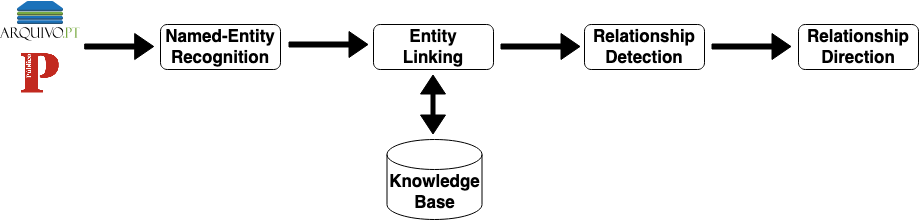
\includegraphics[width=\textwidth,height=4cm]{politiquices_pipeline.png}
%  \caption{Politiquices pipeline for generating RDF triples.}
%  \label{fig:pipeline}
%\end{figure*}

Os componentes descritos na secção anterior formam o processo de extracção de triplos RDF a partir dos títulos de notícias recolhidos do arquivo da web portuguesa, formando assim um grafo que pode ser interrogado recorrendo à linguagem SPARQL.

O processo de extracção começa por fazer o reconhecimento de personalidades no título na notícia e a sua ligação com o identificador de cada personalidade na Wikidata. Para continuar é necessário que as personalidades reconhecidas sejam ligadas com a Wikidata, e se assim for detecta o tipo de relação presente no título.  Se a relação entre as personalidades no título da notícia não for classificada como \textbf{outra} o classificador da direcção da relação é também aplicado ao título. 

Para todos os títulos não descartados em nenhuma etapa do processo, o resultado final é um triplo RDF, ligando personalidades representadas na Wikidata através de uma relação de oposição ou apoio suportada por uma notícia.

% descrever

\begin{comment}

% Personalidades
%
% <wiki_URI, SKOS.altLabel, name>
% wd:Q100269161 ns2:altLabel "Henrique Constantino"@pt ;
%    wdt:P31 wd:Q5 .

% Notícias
%  <url, DC.title, title>
%  <url, DC.data, date)

% Relações
%
% _rel = BNode()
% g.add((_rel, ns1.type, Literal(rel.rel_type)))
% g.add((_rel, ns1.score, Literal(rel.rel_score, datatype=XSD.float)))
% g.add((_rel, ns1.url, URIRef(rel.url)))
% g.add((_rel, ns1.ent1, URIRef(f"http://www.wikidata.org/entity/{rel.ent1}")))
% g.add((_rel, ns1.ent2, URIRef(f"http://www.wikidata.org/entity/{rel.ent2}")))
% g.add((_rel, ns1.ent1_str, Literal(rel.ent1_str)))
% g.add((_rel, ns1.ent2_str, Literal(rel.ent2_str)))



\end{comment}

Os triplos RDF gerados são então indexados num motor SPARQL~\citep{jena2015free} juntamente com um sub-grafo da Wikidata descrito na Secção~\ref{sec_kb}.

% ToDo: descrever o grafo final em nós e relações

\begin{table}[!h]
    \begin{center}
    \begin{tabular}{l r}
        \hline
        Personalidades 	 	& 589 \\
		Partidos Políticos	&  86 \\
		Notícias			& \\
			- arquivo.pt	& \\
			- publico.pt    & \\
			- CHAVE			& \\
		\hline
    \end{tabular}
	\caption{Caracterização do grafo.}
	\label{tab:grafo}
	\end{center}
\end{table}

% dar exemplos dos queries que se possam fazer, ver os exemplos
% ToDo: links para o site com a demo
% availabe to download under the Turtle format https://www.w3.org/TR/turtle/

\begin{comment}
%  ner_linked.jsonl
%  titles_processed.jsonl
%  titles_processed_more_entities.jsonl
%  titles_processed_no_wiki_id.jsonl

% ToDo: qnts nao têm named-entities?
% 	ner_ignored.jsonl
% 	titles_processed_no_entities.jsonl

% ToDo: entities but not found on Wikidata
% 	 no_wiki_id.jsonl
\end{comment}


\section{Trabalho Futuro}
\label{sec:future_work}

% Review the dataset

% - mostrar mais relações:
%    - apoia/defende c/ as duas direções
%    - acusa/opoem-se c/ as duas direções
%        e.g: "Sócrates e Alegre trocam acusações sobre co-incineração"
%			  "Pinto da Costa rebate críticas de Pacheco Pereira"

% analisar tb títulos com mais do que 2 entidades

% limitações das datas, são as datas de crawl e não de publicação da notícia, como combater isto?

% algumas relações/sentimento são dificeis de extraiar:
%	- requerem contexto
%	- usam expressoes idiomáticas ou irónicas


\begin{comment}
	% ent1 asks for action from ent2
	% Jorge Coelho apela a Guterres que apresente candidatura à Presidência da República
	% Narana Coissoró espera que Cavaco "se lembre" do apoio dado pelo CDS
	% Jaime Gama espera de Cavaco Silva "disponibilidade e cooperação"
	% Paulo Portas apela a Cavaco Silva para que vete a lei de execução de penas
	% Paulo Rangel propõe a Sócrates activação do fundo de solidariedade da UE
	% Jorge Lacão sugere que Ferreira Leite vá depor à comissão de inquérito
	% Fernando Nobre não pediu voto a Mário Soares, mas ficaria “honrado com o seu apoio”
	% Obama diz a Mubarak que a transição política “tem que começar agora”
	% Mário Soares pede intervenção de Cavaco para “impedir uma catástrofe”
	% Narciso Miranda pede a Sócrates que renuncie à recandidatura a primeiro-ministro
	% Santos Silva admite que Cavaco deve mediar negociações
	% Passos pede a Sócrates “todas as análises” realizadas pela “troika”
	% César apela Cavaco para impedir medidas alegadamente inconstitucionais
	% Zorrinho espera que Cavaco continue a apelar à “sensibilidade do Governo”
	% Seguro espera que Merkel traga investimento
	% Jorge Miranda aconselha Cavaco a pedir fiscalização do Orçamento
	% António Arnaut entende que Seguro deve convocar congresso
	% Passos assume que pediu a Cavaco para enviar medidas para o TC
	% Cavaco pediu a Ban Ki-Moon reunião internacional para pressionar Guiné-Bissau
	% Paulo Morais apela a Eduardo dos Santos para libertar activistas
	% Catarina Martins pede a Costa que reconsidere escolha do novo chefe das secretas
\end{comment}

% Julgo que os resultados do Politiquices representam um complemento importante nos recursos já existentes para o processamento de linguagem natural em Português, mas também um ponto de partida no desafio de fazer análise de sentimento entre personalidades políticas expressas em notícias.

% O grafo de relações permite a cientistas de áreas como: sociologia, ciência política e computação realizar diversos estudos, por exemplo:

% Encontrar comunidades de apoio e oposição em função do tempo e verificar se há mudanças entre alianças e oposições

% Enriquecer as relações, categorizando-as num ou mais tópicos com base numa análise detalhada do texto da notícia

% Estudar os triângulos políticos: se as personalidades políticas X e Y sempre acusam ou defendem uma terceira personalidade Z, qual será a relação típica entre X e Y ?

% Os dados anotados permitem que novos algoritmos sejam treinados para detectar relações e ligar as personalidades com a Wikidata, e servem de incentivo ao desenvolvimento de melhores algoritmos de processamento de linguagem natural no contexto de notícias de âmbito político em Português.

% O grafo de relações permite a cientistas de áreas como: sociologia, ciência política e computação realizar diversos estudos, por exemplo: 

	% Encontrar comunidades de apoio e oposição em função do tempo e verificar se há  mudanças entre alianças e oposições

	% Enriquecer as relações, categorizando-as num ou mais tópicos com base numa análise detalhada do texto da notícia

	% Estudar os triângulos políticos: se as personalidades políticas X e Y sempre acusam ou defendem uma terceira personalidade Z, qual será a relação típica entre X e Y ?


\newpage


\section*{Agradecimentos}

% Os agradecimentos devem ser colocados sempre numa secção final, sem número, tal como neste exemplo. Sempre que o autor assim o entender, deverá agradecer aos revisores.

\bibliography{references.bib}


\end{document}
